\documentclass{article}
\usepackage[utf8]{inputenc}
\usepackage{amsfonts}
\usepackage{amsmath}
\usepackage{graphicx}
\usepackage[a4paper, total={6in, 8in}]{geometry}
\usepackage{setspace}
\usepackage{enumitem}
\usepackage{xparse}
\usepackage{tkz-tab}


\everymath{\displaystyle}

\newcommand\tab[1][1cm]{\hspace*{#1}}
\doublespacing
\author{Frederic Becerril}

\NewDocumentCommand{\mylim}{ O{n} O{\infty}}{\underset{#1 \rightarrow #2}{\longrightarrow}}
\newcommand{\mysim}[2]{\underset{#1 \rightarrow #2}{\sim}}
\newcommand{\mysupp}[1]{\underset{x \in #1}{Sup}}

\begin{document}

\part*{Exerice 3}

$f_n(x) = \frac{1}{1 + nx^2}$\\
$\bullet$ Soit $x \in \mathbb{R}_+$ on a que\\
si $x \neq 0$ $\frac{1}{1 + nx^2} \mylim 0$\\
Si $x = 0$ $\frac{1}{1 + n0^2} = 1 \mylim 1$\\
Donc $f_n$ converge simplement vers la fonction f := $\left\{
\begin{array}{ll}
    0 \mbox{ si } x > 0\\
    1 \mbox{ sinon}
\end{array}
\right.$\\
$\bullet$ $f_n(x)' = -\frac{2nx}{(1 + nx^2)^2}$\\
Or $-2nx \leq 0$ et $(1 + nx^2)^2 \geq 0$ donc $f_n(x)' \leq 0$\\
$f_n(0) = 1$\\
$f_n(x) \mylim[x][\infty] = 0$\\
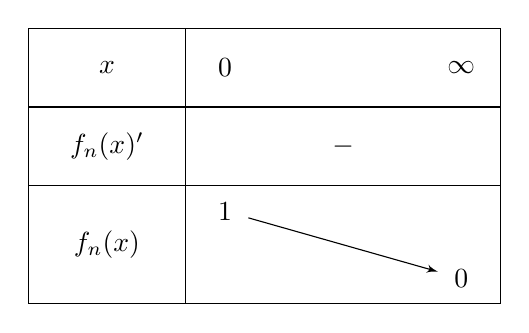
\begin{tikzpicture}
    \tkzTabInit{$x$ / 1 , $f_n(x)'$ / 1, $f_n(x)$ / 1.5}{$0$, $\infty$}
    \tkzTabLine{, -, }
    \tkzTabVar{+/ 1, -/ 0,}
\end{tikzpicture}\\
On a donc que $||f_n(x) - f(x)||_\infty = \mysupp{\mathbb{R}_+} |f_n(x) - f(x)|$\\
\underline{Cas 1}: x = 0 on $|f_n(0) - f(0)| = 1 - 1 = 0$\\
\underline{Cas 2}: $x \neq 0$ on a $\mysupp{\mathbb{R}^*_+} |f_n(x) - f(x)| = \mysupp{\mathbb{R}^*_+} |f_n(x)|$\\
Car si $x \neq 0$ on a $f(x) = 0$\\
Donc $|f_n(x) - f(x)||_\infty = \mysupp{\mathbb{R}^*_+} |f_n(x)|$\\
Comme $f_n(x) \mylim[x][0] 1$, on a que $\mysupp{\mathbb{R}^*_+} |f_n(x)| = 1 \neq 0$\\
Donc $f_n$ ne converge pas uniformement vers f sur $\mathbb{R}_+$\\
Soit $a > 0$\\
$|f_n(x) - f(x)||_{\infty, [a, +\infty[}$ = $\mysupp{[a, +\infty[} |f_n(x)| = f_n(a)$\\
Or $f_n(a) \mylim 0$ donc $f_n$ converge uniformement vers f sur $[a, +\infty[$\\

\end{document}